\note{Brief Overview}{
\subsection*{\ref{act1.2.4}	More Practice With the Energy-Interaction Model	 (\about\unit[30]{min})}
\subsubsection*{Purpose}
\begin{itemize}
\item Practice using the energy-interaction model to develop explicit equations, rather than just searching for equations with the correct variables and not understanding why they should be used.
Learning Outcomes:
\item Be able to justify the use of specific phase-change and heat capacity equations from the Energy-Interaction Model energy system diagram for any specific thermal phenomena
\end{itemize}
}
%Not making this a section because it's really just more practice and should be a part of the previous activity
%\section[Quantitative Applications of the Model]{Quantitative Applications of the \EnergyInteractionModel{}}
\label{act1.2.4}

\note{

	\begin{itemize}
		\item Groups 1 - 3 discuss and respond to \ref{FNT1.2.1-6} as directed below.
		\item Groups 4 - 6 discuss and respond to \ref{FNT1.2.1-7} as directed below.
	\end{itemize}

}

\subsection{Boiling Liquid Nitrogen with Ice}  

\note{For \FNT~\thechapter-\ref{FNT1.2.1-6}}{
Don�t let them show all of the algebraic details! The focus should be on using the model (or in this case, the diagram) to interpret the equations. If the students make sense of the presentation illustrated at the right, all that is left is algebra. The point here is not forbidding them from putting stuff up, but on developing their ability to clarify their questions based on this presentation of information. 
\\[0.25in]
They should always check that the sign of the terms matches their diagrams, and that the units and magnitude of the answer makes sense.\\
\begin{center}
\label{bondsmeltinginice}
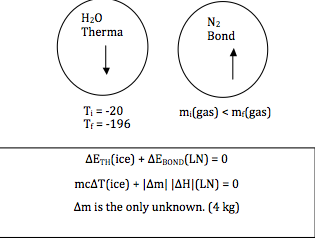
\includegraphics[width=0.6\linewidth]{fnt121-6}
\end{center}
}
\begin{FNTenv}
	\input{U1/FNT1.2.1-6}
\end{FNTenv}

\note{Timing: \unit[\about10]{min}}{
	
}

\begin{enumerate}
	\item There exists a definite correlation between each energy system in your \EnergyDiagram{} and each $\Delta E$ term in your energy conservation equation. In addition to ensuring that you include all the appropriate $\Delta E$'s (and no extra ones) in your algebraic equation expressing conservation of energy, what other very important detail can your \EnergyDiagram{} tell you about each $\Delta E$ term in your equation?
	
	\item Construct a complete \EnergyDiagram{} (including an algebraic statement of energy conservation in terms of the $\Delta E$'s) for this process. Then rewrite the equation expressing energy conservation substituting in the appropriate expressions for changes in energy of the energy systems using variables only (no numbers). \textbf{Do not substitute any numbers for the variables, and do not solve for the unknown, but circle the unknown variable in the equation.} Put the algebraic sign in parentheses above each algebraic term in the algebraic equation.

	We know you know how to do simple algebra and arithmetic. However, the most common mistake students often make is in the algebraic sign of the whole term when subtracting \emph{initial} values from \emph{final} values of the indicators. By using the \EnergyDiagram{} to check that the sign is correct, you will avoid making this error.\footnote{Just for reference: You likely found that \about\unit[4]{kg} of liquid \ce{N2} was converted to vapor.}

\end{enumerate}

\subsection{Warming Ice with Liquid Water}  
\note{For \FNT~\thechapter-\ref{FNT1.2.1-7}}{
\begin{center}
\label{bondsmeltinginice2}
\includegraphics[width=0.6\linewidth]{fnt121-7}
\end{center}
}
\begin{FNTenv}
	\input{U1/FNT1.2.1-7}
\end{FNTenv}

\note{Timing: \unit[\about10]{min}}{}

\begin{enumerate}
	\item Describe in words what is going on in this process, specifically: What physical system is changing phase? What system is changing temperature? What energy systems need to be included in the particular model you create for this process?
	
	\item Construct a complete \EnergyDiagram{} (including an algebraic statement of energy conservation in terms of the $\Delta E$'s) for this process. Then rewrite the equation that expresses energy conservation, substituting in the appropriate expressions for changes in energy of the energy systems using variables only (no numbers). \textbf{Do not substitute any numbers for the variables, and do not solve for the unknown,} but circle the unknown variable in the equation.\footnote{Again, for reference: You likely got a final mass of ice of \about\unit[5]{kg}.}

\WCD

\end{enumerate}

\subsection{Melting Gold}
\note{For \FNT~\thechapter-\ref{FNT1.2.1-8}}{
With a mass specific heat of 0.126 kJ/kg it takes 84.7 kJ to increase the temperature of the solid from 1000 K to the melting point (TMP = 1336 K). 
\\[0.25in]
With a heat of melting of 62.8 kJ/kg, 94.2 kJ must be removed from the liquid to change completely to solid. 
\\[0.25in]
Therefore the solid will reach the melting point before the liquid has completed its phase change, and the final phase will be mixed solid/liquid. 
\\[0.25in]
At the end, suggest that they go home and determine how much liquid changed to solid. [Answer: 1.35 kg changes from liquid to solid] 
}
\begin{FNTenv}
	\input{U1/FNT1.2.1-8}
\end{FNTenv}

\note{Timing: \unit[\textless5]{min}}{
	
}

\noindent Discuss in your group and make sure everyone is prepared to explain your group's response in the whole class discussion.

\WCD
